\documentclass[11pt,a4paper]{article}
\usepackage[utf8]{inputenc}
\usepackage[T1]{fontenc}
\usepackage{lmodern}
\usepackage[margin=2.4cm,top=2.6cm,bottom=2.6cm]{geometry}
\usepackage{amsmath}
\usepackage{graphicx}
\usepackage{booktabs}
\usepackage{xcolor}
\usepackage{caption}
\usepackage{float}
\usepackage{enumitem}
\usepackage{tikz}
\usetikzlibrary{arrows.meta,positioning,shapes.geometric}
\usepackage[hidelinks]{hyperref}
\setlist{itemsep=2pt,topsep=4pt}
\setlength{\parskip}{4pt}
\setlength{\parindent}{0pt}
\captionsetup{font=small,labelfont=bf}
\tikzset{box/.style={draw,rounded corners=3pt,minimum width=3.4cm,minimum height=0.9cm,align=center,font=\small},
arrow/.style={-{Stealth},thick}}

\begin{document}

% ---------------- Title page ----------------
\begin{titlepage}
\centering

\includegraphics[width=3.2cm]{assets/college-logo.jpg}\\[0.6cm]
{\large\bfseries A Course End Project Report on}\\[0.5cm]
{\LARGE\bfseries Online Examination Management System}\\[1.2cm]
{\large Submitted by}\\[0.3cm]
\begin{tabular}{ll}
Vannala Ramcharan & Roll No.\ 25881A05DQ \\
\end{tabular}\\[0.8cm]
{\large Course Facilitator}\\[0.2cm]
{Mr. D. Ganesh}\\[1.2cm]
{\large\bfseries Department of Computer Science and Engineering}\\[0.3cm]
{\large\bfseries Vardhaman College of Engineering, Hyderabad}\\[0.3cm]
{\large\bfseries October 2026}\\[0.5cm]
{\small Project Repository: \url{https://github.com/Ramcharan-v15/online-examination-management-system}}
\vfill
{\small Note: the supplied project list showed this title against three roll numbers.
At the author's instruction, only roll number 25881A05DQ is used in this report;
the other two roll numbers are not reproduced here.}
\end{titlepage}

\tableofcontents
\newpage

\begin{abstract}
\noindent Traditional paper-based examinations are slow to set, slow to mark, and
hard to reuse: question papers must be printed, answer scripts collected, and every
script marked by hand before results can be compiled. This project implements a
console-based \textbf{Online Examination Management System} in plain Java with no
external frameworks, libraries, or database server. An administrator creates exams
and multiple-choice questions; a student registers by roll number, takes an exam
within its time limit, and receives an immediately computed result. Results are
persisted as CSV files so that exams and outcomes survive between runs.
The system was verified by a dependency-free test harness (20 checks, all passing)
and by a scripted demo run that scores 8/10 (80\%, PASS) on a five-question sample
exam. The report documents only features that are actually implemented; authentication,
a graphical interface, and question shuffling are explicitly listed as future work,
not claimed as present.

\noindent\textbf{Keywords:} online examination, Java, console application, multiple-choice
assessment, automated scoring, CSV persistence.
\end{abstract}

\section{Introduction and Problem Statement}
Examinations are a core assessment activity in colleges, yet a fully manual process
has well-known costs. Setting a paper, distributing it, invigilating, collecting
scripts, marking them, totalling marks, and compiling a result sheet are separate
manual steps, each of which can introduce delay or transcription error. A student
typically waits days for a result that a computer could compute the moment the last
answer is submitted.

The problem addressed here is narrower and deliberately so: provide a small,
dependable tool for creating a multiple-choice exam, administering it to students
on one machine, scoring it automatically, and keeping a durable record of results.
The tool is aimed at classroom use, practice tests, and course-end project
demonstration --- not at high-stakes, remotely proctored examinations, for which
authentication, identity verification, and secure delivery would be essential and
are absent here (see \S\ref{sec:limitations}).

Two facts about the starting point must be stated plainly, because they shape
everything that follows. First, the archive supplied for this task
(\texttt{Course\_End\_Report\_Latex\_Template.zip}) contained only a LaTeX course-end
report template --- for an unrelated electronics project --- and no Java source
code at all. There was therefore no existing exam system to audit, preserve, or
refactor. Second, the project title itself comes from the supplied list (item 6,
``Online Examination Management System''). This implementation was built from
scratch to that title, and the report describes that new code only.

\section{Objectives and Scope}
The objectives of the system are:
\begin{itemize}
\item Let an administrator create exams with a title and a time limit, and add
four-option multiple-choice questions with marks to each exam.
\item Let a student register by roll number, select an exam, answer its questions,
skip questions, and receive an immediate result with score, percentage, and
pass/fail status.
\item Score deterministically: a correct answer earns the question's full marks;
a wrong, skipped, or out-of-range answer earns zero. There is no negative marking.
\item Enforce the exam time limit by auto-submitting an attempt when it expires.
\item Persist exams, questions, students, and results between runs in a human-readable
form, without requiring a database server.
\item Reject invalid input (blank fields, wrong option counts, duplicate ids,
non-numeric menu input) with a clear message instead of crashing.
\item Keep the implementation dependency-free, so that it builds with a plain JDK.
\end{itemize}
Out of scope, by design: user passwords and authentication, a graphical or web
interface, concurrent multi-user access, question shuffling, and remote proctoring.
These are future work (\S\ref{sec:future}), not hidden omissions.

\section{Requirements and Technology Stack}
Table~\ref{tab:stack} lists what the system actually uses. The choice of plain Java
and CSV files is a deliberate trade-off: it removes installation friction and
external failure modes for a classroom project, at the cost of the scalability and
concurrency a database would provide.

\begin{table}[H]
\centering
\caption{Technology stack as implemented.}
\label{tab:stack}
\begin{tabular}{@{}ll@{}}
\toprule
\textbf{Item} & \textbf{Choice} \\
\midrule
Language & Java (plain, no frameworks) \\
User interface & Console (standard input/output) \\
Build & \texttt{javac} / \texttt{java} directly; scripts \texttt{run.sh}, \texttt{run\_tests.sh} \\
Storage & CSV files under \texttt{data/} (\texttt{exams.csv}, \texttt{questions.csv}, \\
& \texttt{students.csv}, \texttt{results.csv}) \\
Testing & Dependency-free harness in \texttt{tests/} (no JUnit) \\
External dependencies & None \\
\bottomrule
\end{tabular}
\end{table}

Functional requirements are: (FR1) create/list exams; (FR2) add questions to an
exam; (FR3) register a student; (FR4) take an exam and auto-submit on timeout;
(FR5) compute and display a result; (FR6) list results per exam and per student;
(FR7) persist and reload all data. Non-functional requirements are: the program
must build with a single JDK, start without configuration, never crash on
malformed menu input, and keep every data file readable in a text editor.

\section{System Design}
\subsection{Architecture}
Figure~\ref{fig:arch} shows the layered structure. The console UI never touches
files directly: it calls services, services operate on model objects, and only the
store layer reads and writes CSV. This separation is what makes the scoring logic
testable without any user interface --- the test harness exercises
\texttt{QuizEngine} directly.

\begin{figure}[H]
\centering
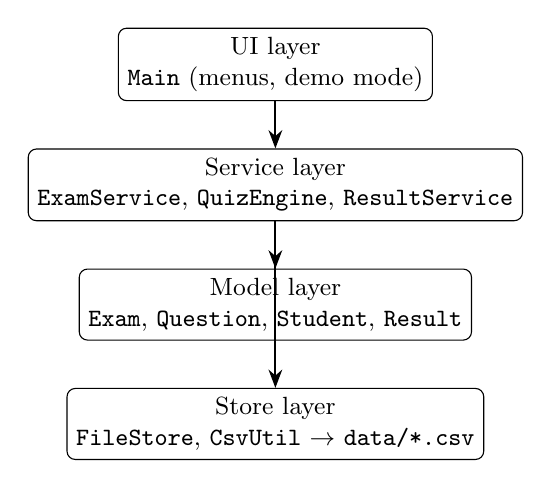
\begin{tikzpicture}[node distance=0.6cm]
\node[box] (ui) {UI layer\\ \texttt{Main} (menus, demo mode)};
\node[box,below=of ui] (svc) {Service layer\\ \texttt{ExamService}, \texttt{QuizEngine}, \texttt{ResultService}};
\node[box,below=of svc] (model) {Model layer\\ \texttt{Exam}, \texttt{Question}, \texttt{Student}, \texttt{Result}};
\node[box,below=of model] (store) {Store layer\\ \texttt{FileStore}, \texttt{CsvUtil} $\rightarrow$ \texttt{data/*.csv}};
\draw[arrow] (ui) -- (svc);
\draw[arrow] (svc) -- (model);
\draw[arrow] (svc) -- (store);
\end{tikzpicture}
\caption{Layered architecture. Arrows show the direction of calls.}
\label{fig:arch}
\end{figure}

\subsection{Modules and classes}
Table~\ref{tab:modules} summarises each class and its single responsibility.
Validation lives in the model constructors, so an invalid object cannot be
constructed anywhere in the program --- not just in the UI path. For example,
\texttt{Question} requires exactly four non-blank options, a correct index in
0--3, and positive marks; \texttt{Exam} requires a positive duration;
\texttt{Result} requires $0 \le \text{score} \le \text{maxMarks}$.

\begin{table}[H]
\centering
\caption{Classes and responsibilities.}
\label{tab:modules}
\begin{tabular}{@{}p{3.6cm}p{9.6cm}@{}}
\toprule
\textbf{Class} & \textbf{Responsibility} \\
\midrule
\texttt{model.Question} & One MCQ: text, four options, correct index (0-based), marks. \\
\texttt{model.Exam} & Id, title, duration, ordered question list; rejects duplicate question ids. \\
\texttt{model.Student} & Roll number (the login key) and name. \\
\texttt{model.Result} & Immutable outcome; percentage and pass/fail at a 40\% threshold. \\
\texttt{service.ExamService} & Exam registry; rejects duplicate exam ids; supplies the sample exam. \\
\texttt{service.QuizEngine} & Pure scoring function (see \S\ref{sec:impl}). \\
\texttt{service.ResultService} & Result list with per-exam, per-student, and average queries. \\
\texttt{store.CsvUtil} & Minimal RFC-4180-style CSV quoting and parsing, no library. \\
\texttt{store.FileStore} & Loads/saves the four CSV files; skips malformed lines on load. \\
\texttt{ui.Main} & Menus, input reprompting, time-limit enforcement, \texttt{--demo} mode. \\
\bottomrule
\end{tabular}
\end{table}

\subsection{Exam workflow}
Figure~\ref{fig:flow} shows the two roles. An administrator's work must precede a
student's: an exam with no questions cannot be taken, and the program says so
explicitly rather than scoring an empty attempt.

\begin{figure}[H]
\centering
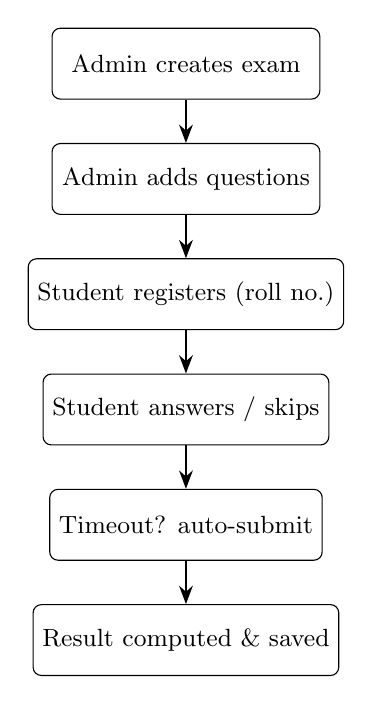
\begin{tikzpicture}[node distance=0.55cm]
\node[box] (a1) {Admin creates exam};
\node[box,below=of a1] (a2) {Admin adds questions};
\node[box,below=of a2] (s1) {Student registers (roll no.)};
\node[box,below=of s1] (s2) {Student answers / skips};
\node[box,below=of s2] (s3) {Timeout? auto-submit};
\node[box,below=of s3] (s4) {Result computed \& saved};
\draw[arrow] (a1) -- (a2);
\draw[arrow] (a2) -- (s1);
\draw[arrow] (s1) -- (s2);
\draw[arrow] (s2) -- (s3);
\draw[arrow] (s3) -- (s4);
\end{tikzpicture}
\caption{End-to-end workflow, admin role followed by student role.}
\label{fig:flow}
\end{figure}

\section{Implementation Details}
\label{sec:impl}
\subsection{Scoring algorithm}
Scoring is a single linear pass over the exam's questions, implemented in
\texttt{QuizEngine.score()}. For each question $i$, the student's answer (if any)
is compared with the stored correct index; equality adds the question's marks,
anything else adds zero. Answers beyond the question count are ignored, missing
answers count as skipped, and out-of-range values are treated as wrong rather
than throwing an exception. The pass mark is 40\% of the exam total. Complexity is
$O(n)$ in the number of questions, with $O(1)$ extra space --- trivially fast for
classroom-sized exams, and, more importantly, easy to reason about and test.

\subsection{Persistence format}
\texttt{FileStore} writes one header row plus one row per record to each CSV file.
Question text and options are quoted when they contain commas or quotes, so a
question such as ``Which of these, if any, is correct?'' round-trips exactly; this
is covered by a test (see \S\ref{sec:testing}). On load, a missing
\texttt{data/} directory simply means ``first run''; a malformed line is skipped
rather than aborting the whole load, and duplicate ids encountered on load are
likewise skipped. The data directory can be overridden with the
\texttt{OEMS\_DATA} environment variable, which is how tests and demos avoid
clobbering a user's real data.

\subsection{Input validation and time limit}
All menu input is read as text and parsed; a non-numeric entry or a number
outside the offered range reprompts instead of crashing (a common failure mode
of naive \texttt{Scanner.nextInt()} code, which this program avoids by reading
whole lines). During an attempt, the start time is recorded and checked before
each question; once the elapsed time reaches the exam duration, the attempt is
submitted with the answers given so far. The timer is checked per question, not
per keystroke, which is a stated limitation of the console design.

\subsection{Sample exam}
The built-in sample exam \texttt{JAVA101 -- Java Fundamentals} (30 minutes,
5 questions, 10 marks) covers inheritance (\texttt{extends}), primitive types,
\texttt{int} size, \texttt{HashSet} uniqueness, and the \texttt{main()} entry
point. It exists so that the program can be demonstrated and verified without
first hand-entering data, and it is the exam used in the screenshots and the
demo result below.

\section{User Interface and Screenshots}
The interface is a text menu with two roles (Figure~\ref{fig:menu}). There is no
graphical window to screenshot, so the evidence in this section is genuine
terminal output from real runs of the program, rendered as images. Nothing has
been retyped or edited to imply behaviour the program does not have.

\begin{figure}[H]
\centering
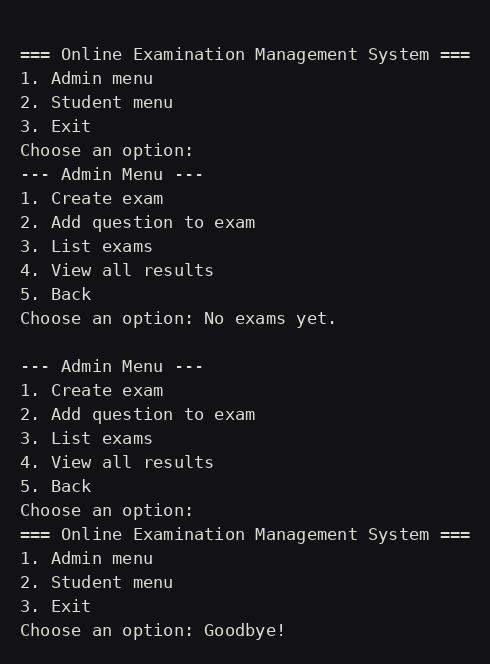
\includegraphics[width=0.62\linewidth]{assets/screenshot-menu.png}
\caption{Main menu and admin menu from a real run (empty data directory, so
listing exams reports ``No exams yet.''). The menu offers the admin menu, the
student menu, and exit; saved data is loaded before the menu appears.}
\label{fig:menu}
\end{figure}

\begin{figure}[H]
\centering
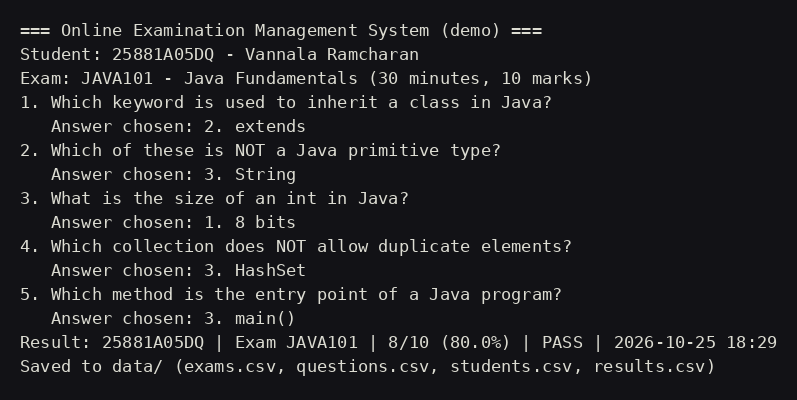
\includegraphics[width=0.92\linewidth]{assets/screenshot-result.png}
\caption{Scripted demo attempt (\texttt{--demo}): the sample exam, the answers
chosen, and the computed result 8/10 (80\%, PASS), followed by confirmation
that the CSV files were saved.}
\label{fig:result}
\end{figure}

A full interactive session follows the same pattern: the admin creates an exam
and adds questions, the student registers, selects the exam id, answers each
question with 1--4 (or 0 to skip), and sees the result line immediately. Invalid
exam ids and empty exams produce explicit error messages, verified by hand
during testing (see \S\ref{sec:testing}).

\section{Testing}
\label{sec:testing}
\subsection{Methodology}
Two kinds of verification were used. First, an automated harness
(\texttt{tests/com/oems/TestRunner.java}) with 20 checks, run by
\texttt{run\_tests.sh}. It uses no test framework, because the project has no
dependencies by design; each check prints PASS or FAIL and the process exits
non-zero if any check fails. Second, manual end-to-end runs: the interactive
menu, the scripted demo, and invalid-input cases (non-numeric menu input,
unknown exam id, empty exam) were exercised by actually running the program.

\subsection{Test cases and results}
Table~\ref{tab:tests} groups the automated checks. All 20 passed in the final
run; the harness output is reproduced in the project repository alongside the
code. The demo run independently confirms the scoring path end to end: answers
(correct, correct, wrong, correct, correct) on five 2-mark questions give
$4 \times 2 = 8$ out of 10, i.e.\ 80\%, PASS --- exactly what the program printed
(Figure~\ref{fig:result}). Edge cases verified by hand include: entering text
where a number was expected (reprompt, no crash), selecting a non-existent exam
(error message, return to menu), and attempting an exam with no questions
(error message, no result recorded).

\begin{table}[H]
\centering
\caption{Automated test groups (20 checks total).}
\label{tab:tests}
\begin{tabular}{@{}p{4.2cm}p{7.2cm}c@{}}
\toprule
\textbf{Group} & \textbf{What is checked} & \textbf{Result} \\
\midrule
Scoring (7) & All correct 10/10; demo answers 8/10; no answers 0/10 FAIL; & 7/7 pass \\
& out-of-range answers treated as wrong; 40\% boundary passes & \\
Validation (8) & 3-option question, bad correct index, 0 marks, 0 duration, & 8/8 pass \\
& blank roll number, duplicate exam id, unknown exam, & \\
& duplicate question id --- all rejected & \\
Result queries (4) & Per-exam filter, per-student filter, average 90.0\%, & 4/4 pass \\
& average of unknown exam 0.0\% & \\
CSV (1) & Quoting round-trips commas and quotes in text & 1/1 pass \\
\midrule
\textbf{Total} & & \textbf{20/20 pass} \\
\bottomrule
\end{tabular}
\end{table}

No test was written for a feature that does not exist, and no result in this
section is estimated: the counts above are the harness's own output, and the
demo score is the program's own printed output.

\section{Limitations and Future Improvements}
\label{sec:limitations}
\label{sec:future}
The honest limitations are: (1) no authentication --- anyone who knows a roll
number can take an exam as that student, so this build is unsuitable for
high-stakes assessment as it stands; (2) no graphical or web interface;
(3) CSV storage is single-writer and will not scale to concurrent users;
(4) the time limit is enforced between questions, not continuously; (5) questions
are presented in fixed order with no shuffling, so neighbouring students see the
same order; (6) no facility for descriptive/essay answers, partial credit, or
negative marking.

Plausible future work, in priority order: password-based login with admin and
student roles; a database (e.g.\ SQLite or MySQL) replacing CSV files;
question and option shuffling per attempt; a Swing/JavaFX or web front end;
result export to PDF/Excel; and an admin dashboard with per-question statistics.
Each of these is future work only --- none is described anywhere in this report
as already implemented.

\section{Conclusion}
This project delivers a working, dependency-free Online Examination Management
System in Java: administrators create exams and questions, students take exams
under a time limit, scoring is immediate and deterministic, and results persist
as readable CSV files. The implementation is small enough to read in full, yet
complete enough to demonstrate the whole examination workflow, and it is verified
by 20 automated checks (all passing) plus real interactive and scripted runs.
Its limits --- above all, the absence of authentication --- are stated plainly
so that a reader can judge where the system is fit to be used and what would
need to change before it could be used for real, high-stakes examinations.

\begin{thebibliography}{9}
\addcontentsline{toc}{section}{References}
\bibitem{oracle-java} Oracle, \textit{Java SE Documentation}, \url{https://docs.oracle.com/javase/}.
\bibitem{oracle-tutorial} Oracle, \textit{The Java Tutorials}, \url{https://docs.oracle.com/javase/tutorial/}.
\bibitem{bloch} J.~Bloch, \textit{Effective Java}, 3rd ed., Addison-Wesley, 2018.
\bibitem{csv-rfc} Y.~Shafranovich, ``Common Format and MIME Type for Comma-Separated Values (CSV) Files,'' RFC 4180, IETF, 2005, \url{https://www.rfc-editor.org/rfc/rfc4180}.
\bibitem{latex} L.~Lamport, \textit{\LaTeX: A Document Preparation System}, 2nd ed., Addison-Wesley, 1994.
\bibitem{project-repo} Online Examination Management System --- source code, tests, screenshots, and this report, \url{https://github.com/Ramcharan-v15/online-examination-management-system}.
\end{thebibliography}

\end{document}
